\documentclass{article}


% \usepackage{arxiv} # uncomment for preprint

\usepackage[utf8]{inputenc} % allow utf-8 input
\usepackage[T1]{fontenc}    % use 8-bit T1 fonts
% \usepackage{hyperref}       % hyperlinks
\usepackage{url}            % simple URL typesetting
\usepackage{booktabs}       % professional-quality tables
\usepackage{amsfonts}       % blackboard math symbols
\usepackage{nicefrac}       % compact symbols for 1/2, etc.
\usepackage{microtype}      % microtypography
\usepackage{lipsum}
\usepackage{graphicx}
\usepackage{subfigure}
\usepackage{amsmath}

\begin{document}

\section*{Datasets}

The \textbf{annthyroid} dataset is derived from the ``Thyroid Disease'' dataset from the UCIMLR\@.
The original data has 7200 instances with 15 categorical attributes and 6 real-valued attributes.
The class labels are ``normal'', ``hypothyroid'', and ``subnormal''.
For anomaly detection, the ``hypothyroid'' and ``subnormal'' classes are combined into 534 outlier instances, and only the 6 real-valued attributes are used.

The \textbf{arrhythmia} dataset is derived from ``Arrhythmia`` dataset from the UCIMLR\@.
The original dataset contains 452 instances with 279 attributes.
There are five categorical attributes which are discarded, leaving this as a 274-dimensional dataset.
The instances are divided into 16 classes.
The eight smallest classes collectively contain 66 instances and are combined into the outlier class.

The \textbf{breastw} dataset is also derived from the ``Breast Cancer Wisconsin (Original)`` dataset.
This is a 9-dimensional dataset containing 683 instances of which 239 represent malignant tumors and are treated as the outlier class.

The \textbf{cardio} dataset is derived from the ``Cardiotocography'' dataset.
The dataset is composed of measurements of fetal heart rate and uterine contraction features on cardiotocograms.
The are each labelled ``normal'', ``suspect'', and ``pathologic'' by expert obstetricians.
For anomaly detection, the ``normal'' class forms the inliers, the ``suspect'' class is discarded, and the ``pathologic'' class is downsampled to 176 instances forming the outliers.
This leaves us with 1831 instances with 21 attributes in the dataset.

The \textbf{cover} dataset is derived from the ``Covertype'' dataset.
The original dataset contains 581,012 instances with 54 attributes.
The dataset is used to predict the type of forest cover solely from cartographic variables.
The instances are labelled into seven different classes.
For outlier detection, we use only the 10 quantitative attributes, type 2 (lodgepole pine) as the inliers, and type 4 (conttonwood/willow) as the outliers.
The remaining classes are discarded.
This leaves us with a 10-dimensional dataset with 286,048 instances of which 2,747 are outliers.

The \textbf{glass} dataset is derived from the ``Glass Identification'' dataset.
The study of classification of types of glass was motivated by criminological investigations where glass fragments left at crime scenes were used as evidence.
This dataset contains 214 instances with nine attributes.
While there are several different types of glass in this dataset, class 6 is a clear minority with only nine instances and, as such, points in class 6 are treated as the outliers while all other classes are treated as inliers.

The \textbf{http} dataset is derived from the original ``KDD Cup 1999'' dataset.
It contains 41 attributes (34 continuous and 7 categorical) which are reduced to 4 attributes (service, duration, src\_bytes, dst\_bytes).
Only the ``service'' attribute is categorical, dividing the data into {http, smtp, ftp, ftp\_data, others} subsets.
Here, only the ``http'' data is used.
The values of the continuous attributes are centered around 0, so they have been log-transformed far away from 0.
The original data contains 3,925,651 attacks in 4,898,431 records.
This smaller dataset is created with only 2,211 attacks in 567,479 records.

The \textbf{ionosphere} dataset is derived from the ``Ionosphere'' dataset.
It consists 351 instances with 34 attributes.
One of the attributes is always 0 and, so, is discarded, leaving us with a 33-dimensional dataset.
The data comes from radar measurements of the ionosphere from a system located in Goose Bay, Labrador.
The data are classified into ``good'' if the radar returns evidence some type of structure in the ionosphere, and ``bad'' if not.
The ``good'' class serves as the inliers and the ``bad'' class serves as the outliers.

The \textbf{lympho} dataset is derived from the ``Lymphography'' dataset.
The data contain 148 instances with 18 attributes.
The instances are labelled ``normal find'', ``metastases'', ``malign lymph'', and ``fibrosis''.
The two minority classes only contain a total of six instances, and are combined to form the outliers.
The remaining 142 instances form the inliers.

The \textbf{mammography} dataset is derived from the original ``Mammography'' dataset provided by Aleksandar Lazarevic.
Its goal is to use x-ray images of human breasts to find calcified tissue as an early sign of breast cancer.
As such, the ``calcification'' class is considered as the outlier class while the ``non-clacification'' class is the inliers.
We have 11,183 instances with 6 attributes, of which 260 are ``calcifications.''

The \textbf{mnist} dataset is derived from the classic ``MNIST'' dataset of handwritten digits.
Digit-zero is considered the inlier class while 700 images of digit-six are the outliers.
Furthermore, 100 pixels are randomly selected as features from the original 784 pixels.

The \textbf{musk} dataset is derived from its namesake in the UCIMLR\@.
It is created from molecules that have been classified by experts as ``musk'' or ``non-musk''.
The data are downsampled to 3,062 instances with 166 attributes.
The ``musk'' class forms the outliers while the ``non-musk'' class forms the inliers.

The \textbf{optdigits} dataset is derived from the ``Optical Recognition of Handwritten Digits'' dataset.
Digits 1--9 form the inliers while 150 samples of digit-zero form the outliers.
This gives us a dataset of 5,216 instances with 64 attributes.

The \textbf{pendigits} dataset is derived from the ``Pen-Based Recognition of Handwritten Digits'' dataset from the UCI Machine Learning Repository.
The original collection of handwritten samples is reduced to 6,870 points, of which 156 are outliers.

The \textbf{pima} dataset is derived from the ``Pima Indians Diabetes'' dataset.
The original dataset presents a binary classification problem to detect diabetes.
This subset was restricted to female patients at least 21 years old of Pima Indian heritage.

The \textbf{satellite} dataset is derived from the ``Statlog (Landsat Satellite)'' dataset.
The smallest three classes (2, 4, and 5) are combined to form the outlier class while the other classes are combined to form the inlier class.
The train and test subsets are combined to produce a of 6,435 instances with 36 attributes.

The \textbf{satimage-2} dataset is also derived from the ``Satlog (Landsat Satellite)'' dataset.
Class 2 is downsampled to 71 instances that are treated as outliers, while all other classes are combined to form an inlier class.
This gives us 5,803 instances with 36 attributes.

The \textbf{shuttle} dataset is derived from the ``Statlog (Shuttle)'' dataset.
This are seven classes in the original dataset.
Here, class 4 is discarded, class 1 is treated as the inliers and the remaining classes, which are comparatively small, form an outlier class.
This gives us 49,097 instances with 9 attributes, of which 3,511 are outliers.

The \textbf{smtp} is also derived from the ``KDD Cup 1999'' dataset.
It is preprocessed in the same way as the \textbf{http} dataset, except that the ``smtp'' service subset is used.
This version of the dataset only contains 95,156 instances with 3 attributes, of which 30 instances are outliers.

The \textbf{thyroid} dataset is also derived from the ``Thyroid Disease'' dataset.
The attribute selection is the same as for the \textbf{annthyroid} dataset but only the 3,772 training instances are used in this version.
The ``hyperfunction'' class, containing 93 instances, is treated as the outlier class, while the other two classes are combined to form an inlier class.

The \textbf{vertebral} dataset is derived from the ``Vertebral Column'' dataset.
6 attributes are derived to represent the shape and orientation of the pelvis and lumbar spine.
Each instance comes from a different patient.
The ``Abnormal (AB)'' class of 210 instances are used as inliers while the ``Normal (NO)'' class is downsampled to 30 instances to be used as outliers.

The \textbf{vowels} dataset is derived from the ``Japanese Vowels'' dataset.
THE UCIMLR presents this data as a multivariate time series of nine speakers uttering two Japanese vowels.
For outlier detection, each frame of each time-series is treated as a separate point.
There are 12 features associated with each time series, and these translate as the attributes for each point.
Data from speaker 1, downsampled to 50 points, form the outlier class/
Speakers 6, 7, and 8 form the outlier class.
The rest of the points are discarded.
This leaves is with 1,456 points in 12 dimensions, of which 50 are outliers.

The \textbf{wbc} dataset is derived from the ``Wisconsin-Breast Cancer (Diagnostics)'' dataset.
The dataset records measurements for breast cancer cases.
The benign class is treated as the inlier class, while the malignant class is downsampled to 21 points and serves as the outlier class.
This leaves us with 278 points in 30 dimensions.

The \textbf{wine} dataset is a collection of results of a chemical analysis of several wines from a region in Italy.
The data contain 129 samples having 13 attributes, and divided into 3 classes.
Classes 2 and 3 form the inliers while class 1, downsampled to 10 instances, is the outlier class.


\begin{table*}[!t]
    \renewcommand{\arraystretch}{1.25}
    \caption{Datasets used for Benchmarks}
    \label{table:methods:benchmarks}
    \centering
    \begin{tabular}{|c|c|c|c|c|}
    \hline
    \textbf{Dataset} & \textbf{Cardinality} & \textbf{\# Dim.} & \textbf{\# Outliers} & \textbf{\% Outliers} \\
    \hline
    annthyroid & 7,200 & 6 & 534 & 7.42 \\
    \hline
    arrhythmia & 452 & 274 & 66 & 15 \\
    \hline
    breastw & 683 & 9 & 239 & 35 \\
    \hline
    cardio & 1,831 & 21 & 176 & 9.6 \\
    \hline
    cover & 286,048 & 10 & 2,747 & 0.9 \\
    \hline
    glass & 214 & 9 & 9 & 4.2 \\
    \hline
    http & 567,479 & 4 & 2,211 & 0.4 \\
    \hline
    ionosphere & 351 & 33 & 126 & 36 \\
    \hline
    lympho & 148 & 18 & 6 & 4.1 \\
    \hline
    mammography & 11,183 & 6 & 260 & 2.32 \\
    \hline
    mnist & 7603 & 100 & 700 & 9.2 \\
    \hline
    musk & 3,062 & 166 & 97 & 3.2 \\
    \hline
    optdigits & 5,216 & 64 & 150 & 3 \\
    \hline
    pendigits & 6,870 & 16 & 156 & 2.27 \\
    \hline
    pima & 768 & 8 & 268 & 35 \\
    \hline
    satellite & 6,435 & 36 & 2036 & 32 \\
    \hline
    satimage-2 & 5,803 & 36 & 71 & 1.2 \\
    \hline
    shuttle & 59,097 & 9 & 3,511 & 7 \\
    \hline
    smtp & 95,156 & 3 & 30 & 0.03 \\
    \hline
    thyroid & 3,772 & 6 & 93 & 2.5 \\
    \hline
    vertebral & 240 & 6 & 30 & 12.5 \\
    \hline
    vowels & 1,456 & 12 & 50 & 3.4 \\
    \hline
    wbc & 278 & 30 & 21 & 5.6 \\
    \hline
    wine & 129 & 13 & 10 & 7.7 \\
    \hline
    \end{tabular}
    \end{table*}


\begin{table*}[!t]
\renewcommand{\arraystretch}{1.25}
\caption{Performance on Train Datasets}
\label{table:results:train-performance}
% \centering
\vskip 0.15in
\begin{center}
\begin{small}
\begin{sc}
\begin{tabular}{|c|c|c|c|c|c|c|}
\hline
\textbf{model} & \textbf{annthyroid} & \textbf{mnist} & \textbf{pendigits} & \textbf{satellite} & \textbf{shuttle} & \textbf{thyroid} \\
\hline
        CHAODA-fast &                0.64 &  \textbf{0.78} &      \textbf{0.94} &      \textbf{0.79} &             0.51 &    \textbf{0.89} \\
\hline
        CHAODA &                0.65 &           0.73 &      \textbf{0.95} &               0.73 &             0.85 &    \textbf{0.89} \\
\hline
                ABOD &                0.50 &           0.60 &               0.53 &               0.51 &             0.54 &             0.50 \\
\hline
        AutoEncoder &                0.69 &           0.67 &               0.58 &               0.63 &             0.94 &             0.88 \\
\hline
                CBLOF &                0.59 &           0.62 &               0.59 &               0.68 &    \textbf{0.99} &             0.87 \\
\hline
                COF &                0.59 &           0.56 &               0.53 &               0.56 &             0.52 &             0.49 \\
\hline
                HBOS &       \textbf{0.84} &           0.53 &               0.52 &               0.62 &             0.74 &             0.86 \\
\hline
        IFOREST &                0.70 &           0.61 &               0.63 &               0.70 &             0.91 &    \textbf{0.91} \\
\hline
                KNN &                0.65 &           0.65 &               0.51 &               0.56 &             0.53 &             0.56 \\
\hline
                LMDD &                0.52 &           0.59 &               0.56 &               0.42 &             0.92 &             0.70 \\
\hline
                LOCI &         \textit{TO} &    \textit{TO} &        \textit{TO} &        \textit{TO} &      \textit{TO} &      \textit{TO} \\
\hline
                LODA &                0.63 &           0.66 &               0.57 &               0.65 &             0.96 &    \textbf{0.90} \\
\hline
                LOF &                0.60 &           0.57 &               0.52 &               0.57 &             0.53 &             0.49 \\
\hline
                MCD &                0.72 &           0.57 &               0.53 &               0.58 &             0.96 &             0.85 \\
\hline
        MOGAAL &                0.46 &    \textit{TO} &               0.67 &               0.59 &      \textit{TO} &             0.49 \\
\hline
                OCSVM &                0.62 &           0.63 &               0.59 &               0.62 &    \textbf{0.97} &             0.78 \\
\hline
                SOD &                0.64 &           0.55 &               0.52 &               0.52 &      \textit{TO} &             0.53 \\
\hline
        SOGAAL &                0.46 &           0.57 &               0.57 &               0.60 &             0.96 &             0.49 \\
\hline
                SOS &                0.50 &           0.52 &               0.52 &               0.47 &      \textit{TO} &             0.50 \\
\hline
                VAE &                0.69 &           0.67 &               0.58 &               0.63 &             0.94 &             0.88 \\
\hline
\end{tabular}
\end{sc}
\end{small}
\end{center}
\vskip -0.1in
\end{table*}


A simple visualization in Figure~\ref{fig:conclusions:umap-embeddings} using UMAP  illustrates two different examples; the anomalies in one dataset, where CHAODA outperforms other methods, appear to be at the edges of a complex manifold (though, clearly, the UMAP projection has distorted the manifold) while in another dataset, where most methods perform fairly comparably, the distribution is less interesting and many anomalies are distributed apparently randomly across it.

\begin{figure*}
   \centering
   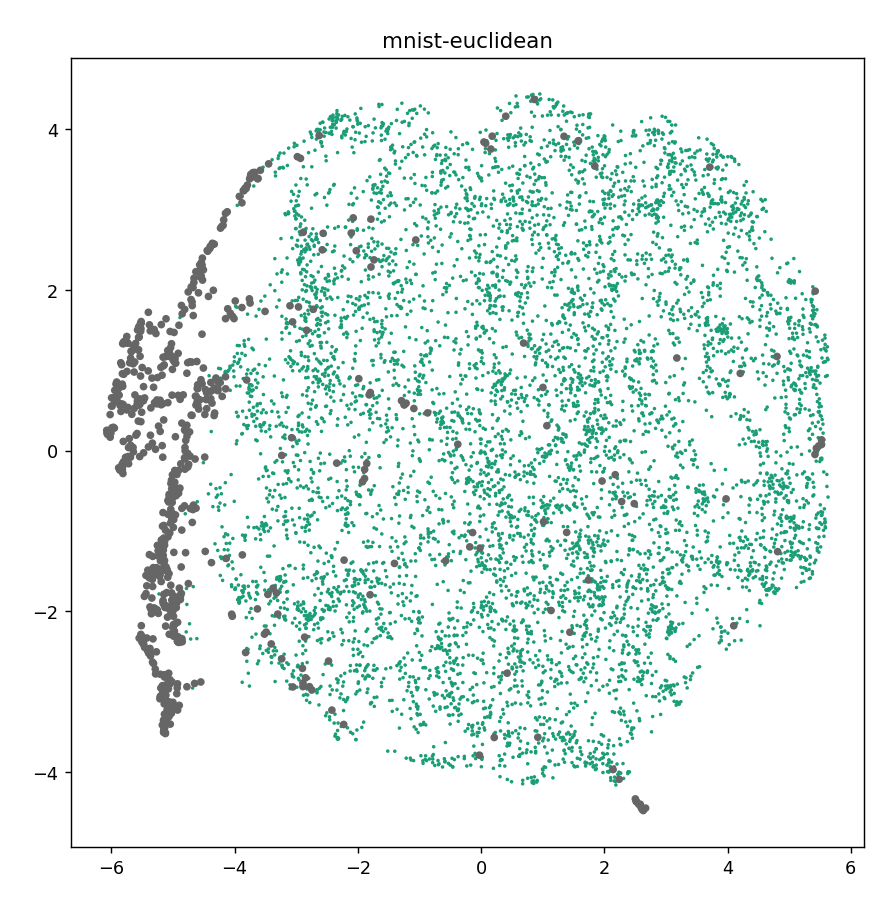
\includegraphics[width=2in]{images/umaps/mnist-euclidean-umap2d.png}
   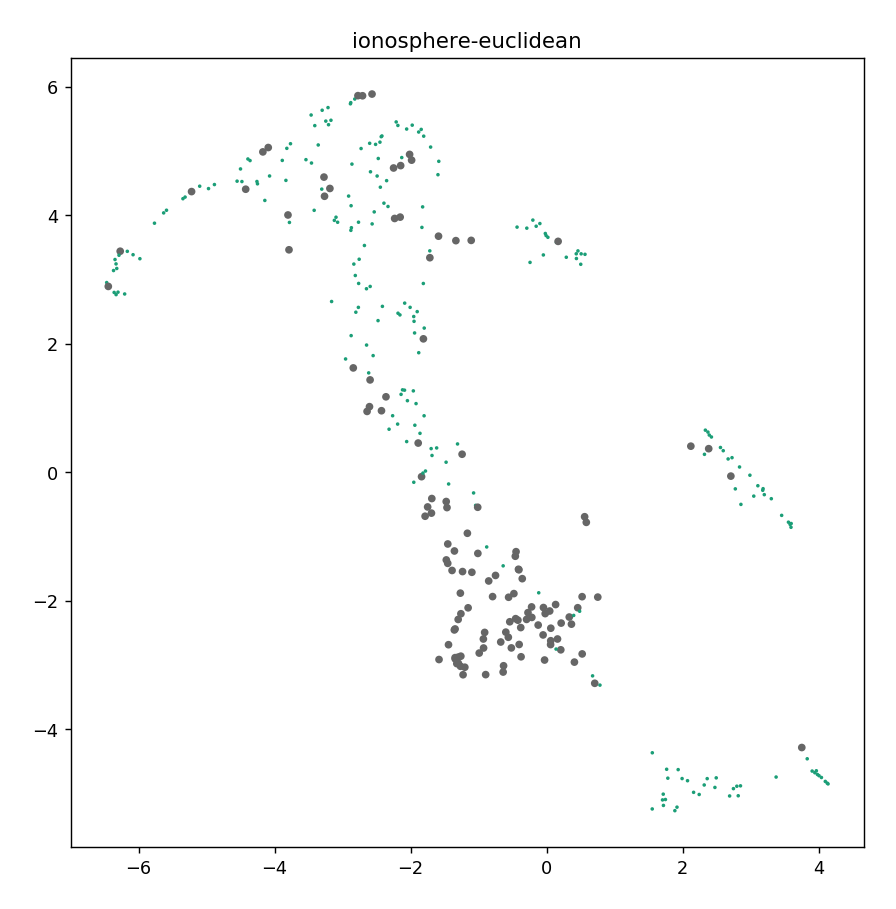
\includegraphics[width=2in]{images/umaps/ionosphere-euclidean-umap2d.png}
   \caption{UMAP projection of MNIST (left) and Ionosphere (right). Anomalies are in gray. Note that for MNIST, the UMAP projection does not find much structure, though most of the anomalies congregate to one side. For Ionosphere, there is a single main component to the manifold, with two more distant clusters, and anomalies tend to be at the edges of a manifold. Most algorithms perform comparably on MNIST, while CHAODA outperforms others on Ionosphere.}
   \label{fig:conclusions:umap-embeddings}
\end{figure*}

% TODO: Add to supplements

\begin{table*}[!t]
\renewcommand{\arraystretch}{1.25}
\caption{Time taken, in seconds, on Train Datasets}
\label{table:results:train-time}
\centering
\begin{tabular}{|c|c|c|c|c|c|c|}
\hline
\textbf{model} & \textbf{annthyroid} & \textbf{mnist} & \textbf{pendigits} & \textbf{satellite} & \textbf{shuttle} & \textbf{thyroid} \\
\hline
        CHAODA-fast &              161.85 &        6221.64 &             617.93 &             425.03 &             5.48 &           117.97 \\
\hline
        CHAODA &              205.74 &       10152.47 &             771.89 &             891.19 &         21415.56 &           219.32 \\
\hline
                ABOD &                3.42 &          16.39 &               2.83 &               3.53 &            21.58 &             1.25 \\
\hline
        AutoEncoder &               22.80 &          40.54 &              23.87 &              26.74 &           158.72 &            12.84 \\
\hline
                CBLOF &                1.01 &           1.14 &               0.23 &               0.30 &             0.71 &             0.21 \\
\hline
                COF &              215.63 &         277.91 &             199.03 &             176.35 &         12106.63 &            54.82 \\
\hline
                HBOS &                1.58 &  \textbf{0.06} &      \textbf{0.01} &      \textbf{0.02} &    \textbf{0.03} &    \textbf{0.00} \\
\hline
        IFOREST &                0.73 &           1.41 &               0.80 &               0.84 &             3.24 &             0.54 \\
\hline
                KNN &                0.84 &          14.30 &               1.25 &               2.05 &             9.13 &             0.42 \\
\hline
                LMDD &              107.05 &        1383.19 &             197.48 &             371.63 &          6274.43 &            32.69 \\
\hline
                LOCI &         \textit{TO} &    \textit{TO} &        \textit{TO} &        \textit{TO} &      \textit{TO} &      \textit{TO} \\
\hline
                LODA &                0.13 &           0.13 &               0.12 &               0.11 &             0.59 &    \textbf{0.08} \\
\hline
                LOF &                0.26 &          14.79 &               0.90 &               1.71 &             6.30 &    \textbf{0.09} \\
\hline
                MCD &                1.50 &          20.56 &               3.01 &              10.39 &            10.78 &             1.03 \\
\hline
        MOGAAL &              594.69 &    \textit{TO} &             561.40 &             513.84 &      \textit{TO} &           280.80 \\
\hline
                OCSVM &                2.70 &          11.30 &               3.04 &               3.83 &           162.18 &             0.68 \\
\hline
                SOD &              262.80 &         281.86 &             195.81 &             253.71 &      \textit{TO} &            91.48 \\
\hline
        SOGAAL &               61.14 &          68.03 &              55.40 &              50.07 &           460.66 &            31.43 \\
\hline
                SOS &              101.82 &          54.22 &              46.02 &              42.62 &      \textit{TO} &            42.10 \\
\hline
                VAE &               27.95 &          50.16 &              29.63 &              33.51 &           182.23 &            16.18 \\
\hline
\end{tabular}
\end{table*}

% TODO: Add to supplements

\begin{table*}[!t]
\renewcommand{\arraystretch}{1.25}
\caption{Time taken, in seconds, on the first half of the Test Datasets}
\label{table:results:test-time-1}
\centering
\begin{tabular}{|c|c|c|c|c|c|c|c|c|c|}
\hline
\textbf{model} & \textbf{arrhythmia} & \textbf{breastw} & \textbf{cardio} & \textbf{cover} & \textbf{glass} & \textbf{http} & \textbf{ionosphere} & \textbf{lympho} & \textbf{mammo} \\
\hline
        CHAODA-fast &                6.70 &             4.71 &          135.17 &        1485.24 &           1.06 &        119.14 &                2.64 &            1.08 &          46.42 \\
\hline
        CHAODA &                6.90 &             4.80 &          143.31 &        3118.26 &           1.10 &        221.81 &                2.78 &            1.74 &          71.54 \\
\hline
                ABOD &                0.34 &             0.20 &            0.72 &          24.02 &  \textbf{0.07} &         19.08 &                0.13 &   \textbf{0.05} &           3.82 \\
\hline
        AutoEncoder &                8.00 &             6.18 &            9.05 &         183.70 &           3.99 &        154.20 &                4.99 &            3.79 &          35.26 \\
\hline
                CBLOF &                0.16 &             0.13 &            0.17 &    \textit{EX} &  \textbf{0.06} &   \textit{EX} &       \textbf{0.07} &   \textbf{0.05} &           0.20 \\
\hline
                COF &                1.24 &             1.84 &           12.63 &       21681.15 &           0.24 &      21228.44 &                0.60 &            0.14 &         513.46 \\
\hline
                HBOS &       \textbf{0.08} &    \textbf{0.00} &   \textbf{0.01} &           1.13 &  \textbf{0.00} & \textbf{0.01} &       \textbf{0.01} &   \textbf{0.01} &  \textbf{0.01} \\
\hline
        IFOREST &                0.43 &             0.34 &            0.43 &           4.61 &           0.30 &          3.95 &                0.33 &            0.30 &           0.95 \\
\hline
                KNN &                0.19 &    \textbf{0.07} &            0.30 &          11.46 &  \textbf{0.02} &          7.47 &       \textbf{0.05} &   \textbf{0.02} &           1.58 \\
\hline
                LMDD &               14.85 &             2.62 &           22.12 &       11579.93 &           0.57 &       3873.99 &                1.73 &            0.42 &         243.01 \\
\hline
                LOCI &              307.04 &      \textit{TO} &     \textit{TO} &    \textit{TO} &          25.68 &   \textit{TO} &              120.92 &            9.78 &    \textit{TO} \\
\hline
                LODA &       \textbf{0.04} &    \textbf{0.03} &   \textbf{0.05} &           0.81 &  \textbf{0.03} &          0.66 &       \textbf{0.03} &   \textbf{0.03} &           0.17 \\
\hline
                LOF &                0.16 &    \textbf{0.01} &            0.18 &          10.24 &  \textbf{0.00} &          1.93 &       \textbf{0.01} &   \textbf{0.00} &           0.59 \\
\hline
                MCD &                5.08 &             0.64 &            0.89 &          28.65 &  \textbf{0.05} &          8.21 &                0.15 &   \textbf{0.05} &           2.11 \\
\hline
        MOGAAL &               46.46 &            42.09 &          116.73 &    \textit{TO} &          40.67 &   \textit{TO} &               40.86 &           37.84 &    \textit{TO} \\
\hline
                OCSVM &       \textbf{0.10} &    \textbf{0.02} &            0.23 &         257.95 &  \textbf{0.00} &        257.28 &       \textbf{0.01} &   \textbf{0.00} &           6.37 \\
\hline
                SOD &                1.19 &             1.89 &           13.39 &    \textit{TO} &           0.31 &   \textit{TO} &                0.76 &            0.20 &         521.25 \\
\hline
        SOGAAL &                6.70 &             5.03 &           14.43 &         591.14 &           3.95 &        597.17 &                4.71 &            3.96 &          92.27 \\
\hline
                SOS &                0.69 &            47.40 &            4.11 &    \textit{TO} &           0.18 &   \textit{TO} &                0.33 &            0.11 &    \textit{TO} \\
\hline
                VAE &               10.00 &             7.75 &           10.89 &         223.09 &           5.27 &        175.59 &                6.66 &            5.21 &          40.87 \\
\hline
\end{tabular}
\end{table*}

% TODO: Add to supplements

\begin{table*}[!b]
\renewcommand{\arraystretch}{1.25}
\caption{Time taken, in seconds, on the second half of the Test Datasets}
\label{table:results:test-time-2}
\centering
\begin{tabular}{|c|c|c|c|c|c|c|c|c|c|}
\hline
\textbf{model} & \textbf{musk} & \textbf{optdigits} & \textbf{pima} & \textbf{satimage-2} & \textbf{smtp} & \textbf{vertebral} & \textbf{vowels} &  \textbf{wbc} & \textbf{wine} \\
\hline
        CHAODA-fast &        858.15 &            3279.67 &         12.36 &              358.49 &        272.61 &               1.88 &          123.34 &          5.26 &          0.39 \\
\hline
        CHAODA &        982.25 &            5865.12 &         13.50 &              611.14 &        451.74 &               2.21 &          181.91 &          6.10 &          0.40 \\
\hline
                ABOD &          4.39 &               6.81 &          0.26 &                3.20 &         18.00 &      \textbf{0.08} &            0.51 &          0.14 & \textbf{0.04} \\
\hline
        AutoEncoder &         23.40 &              24.29 &          4.65 &               23.73 &        195.61 &               2.85 &            6.98 &          4.70 &          3.31 \\
\hline
                CBLOF &          0.27 &               0.44 & \textbf{0.08} &                0.31 &          0.65 &      \textbf{0.06} &   \textbf{0.10} & \textbf{0.08} & \textbf{0.05} \\
\hline
                COF &         45.60 &             119.57 &          2.40 &              141.84 &      21283.99 &               0.28 &            8.06 &          0.68 &          0.11 \\
\hline
                HBOS & \textbf{0.07} &      \textbf{0.04} & \textbf{0.00} &       \textbf{0.02} & \textbf{0.01} &      \textbf{0.00} &   \textbf{0.01} & \textbf{0.01} & \textbf{0.00} \\
\hline
        IFOREST &          0.93 &               0.92 &          0.35 &                0.79 &          3.90 &               0.30 &            0.40 &          0.33 &          0.29 \\
\hline
                KNN &          3.50 &               5.53 & \textbf{0.09} &                1.84 &          6.83 &      \textbf{0.03} &            0.18 & \textbf{0.05} & \textbf{0.01} \\
\hline
                LMDD &        375.11 &             421.22 &          2.86 &              302.94 &       3872.57 &               0.59 &            9.47 &          1.91 &          0.33 \\
\hline
                LOCI &   \textit{TO} &        \textit{TO} &   \textit{TO} &         \textit{TO} &   \textit{TO} &              35.97 &     \textit{TO} &        154.49 &          6.84 \\
\hline
                LODA & \textbf{0.07} &      \textbf{0.10} & \textbf{0.04} &       \textbf{0.10} &          0.73 &      \textbf{0.03} &   \textbf{0.05} & \textbf{0.04} & \textbf{0.03} \\
\hline
                LOF &          3.59 &               5.49 & \textbf{0.02} &                1.50 &          1.36 &      \textbf{0.00} &   \textbf{0.06} & \textbf{0.01} & \textbf{0.00} \\
\hline
                MCD &         84.74 &               7.24 &          0.69 &                6.83 &         13.78 &      \textbf{0.05} &            0.81 &          0.11 & \textbf{0.05} \\
\hline
        MOGAAL &        267.93 &             415.02 &         40.89 &              463.18 &   \textit{TO} &              39.86 &           80.35 &         40.65 &         38.10 \\
\hline
                OCSVM &          2.51 &               3.71 & \textbf{0.03} &                3.14 &        252.52 &      \textbf{0.00} &            0.11 & \textbf{0.01} & \textbf{0.00} \\
\hline
                SOD &         56.94 &             131.49 &          2.48 &              210.39 &   \textit{TO} &               0.54 &           13.92 &          1.03 &          0.19 \\
\hline
        SOGAAL &         29.55 &              44.72 &          5.20 &               48.79 &        592.27 &               4.69 &           10.38 &          4.76 &          4.01 \\
\hline
                SOS &          9.37 &              26.09 &          1.01 &               34.96 &   \textit{TO} &               0.21 &            2.81 &          0.36 & \textbf{0.10} \\
\hline
                VAE &         30.38 &              30.58 &          5.67 &               30.41 &        176.84 &               4.03 &           10.46 &          5.33 &          4.62 \\
\hline
\end{tabular}
\end{table*}


% TODO: Add the following tables to the supplementary materials.


% \subsection{New CHAODA Results}
% \label{subsec:results:new-chaoda-results}

% \begin{table*}[!b]
%     \renewcommand{\arraystretch}{1.25}
%     \caption{New CHAODA Results. Set 1}
%     \label{table:results:new-chaoda-1}
%     \centering
%     \begin{tabular}{|c|c|c|c|c|c|c|c|c|c|}
%         \hline
%         \textbf{voting} & \textbf{normed} & \textbf{\textbf{annthyroid}} & \textbf{\textbf{arrhythmia}} & \textbf{\textbf{breastw}} & \textbf{\textbf{cardio}} & \textbf{\textbf{cover}} & \textbf{\textbf{glass}} & \textbf{\textbf{http}} & \textbf{\textbf{ionosphere}} \\
%         \hline
%                    mean &            None &                \textbf{0.64} &                \textbf{0.77} &             \textbf{0.97} &            \textbf{0.81} &                    0.71 &                    0.70 &          \textbf{1.00} &                \textbf{0.88} \\
%         \hline
%                 product &            None &                         0.62 &                \textbf{0.77} &                      0.92 &                     0.76 &                    0.71 &                    0.63 &          \textbf{1.00} &                         0.80 \\
%         \hline
%                  median &            None &                         0.51 &                         0.57 &                      0.95 &                     0.55 &                    0.49 &                    0.53 &          \textbf{1.00} &                         0.60 \\
%         \hline
%                     min &            None &                         0.61 &                         0.73 &             \textbf{0.98} &            \textbf{0.79} &                    0.71 &                    0.69 &          \textbf{1.00} &                \textbf{0.87} \\
%         \hline
%                     max &            None &                         0.62 &                \textbf{0.75} &             \textbf{0.96} &            \textbf{0.81} &                    0.73 &           \textbf{0.73} &          \textbf{1.00} &                \textbf{0.88} \\
%         \hline
%                     p25 &            None &                \textbf{0.65} &                \textbf{0.75} &             \textbf{0.96} &            \textbf{0.80} &                    0.45 &                    0.70 &          \textbf{1.00} &                \textbf{0.87} \\
%         \hline
%                     p75 &            None &                         0.51 &                         0.74 &             \textbf{0.98} &                     0.73 &           \textbf{0.77} &           \textbf{0.75} &          \textbf{1.00} &                         0.61 \\
%         \hline
%                    mean &          linear &                         0.58 &                \textbf{0.75} &             \textbf{0.98} &            \textbf{0.79} &                    0.74 &           \textbf{0.73} &          \textbf{1.00} &                         0.85 \\
%         \hline
%                 product &          linear &                         0.61 &                         0.73 &             \textbf{0.98} &            \textbf{0.79} &                    0.71 &                    0.69 &          \textbf{1.00} &                \textbf{0.87} \\
%         \hline
%                  median &          linear &                         0.62 &                \textbf{0.75} &             \textbf{0.96} &            \textbf{0.81} &                    0.73 &           \textbf{0.73} &          \textbf{1.00} &                \textbf{0.88} \\
%         \hline
%                     min &          linear &                \textbf{0.65} &                \textbf{0.75} &             \textbf{0.96} &            \textbf{0.80} &                    0.45 &                    0.70 &          \textbf{1.00} &                \textbf{0.87} \\
%         \hline
%                     max &          linear &                         0.51 &                         0.74 &             \textbf{0.98} &                     0.73 &           \textbf{0.77} &           \textbf{0.75} &          \textbf{1.00} &                         0.61 \\
%         \hline
%                     p25 &          linear &                \textbf{0.64} &                \textbf{0.77} &             \textbf{0.97} &            \textbf{0.81} &                    0.71 &                    0.70 &          \textbf{1.00} &                \textbf{0.88} \\
%         \hline
%                     p75 &          linear &                         0.62 &                \textbf{0.77} &                      0.92 &                     0.76 &                    0.71 &                    0.63 &          \textbf{1.00} &                         0.80 \\
%         \hline
%                    mean &        gaussian &                         0.62 &                \textbf{0.75} &             \textbf{0.96} &            \textbf{0.81} &                    0.73 &           \textbf{0.73} &          \textbf{1.00} &                \textbf{0.88} \\
%         \hline
%                 product &        gaussian &                \textbf{0.65} &                \textbf{0.75} &             \textbf{0.96} &            \textbf{0.80} &                    0.45 &                    0.70 &          \textbf{1.00} &                \textbf{0.87} \\
%         \hline
%                  median &        gaussian &                         0.51 &                         0.70 &             \textbf{0.98} &                     0.73 &           \textbf{0.77} &           \textbf{0.75} &          \textbf{1.00} &                         0.61 \\
%         \hline
%                     min &        gaussian &                \textbf{0.64} &                \textbf{0.77} &             \textbf{0.97} &            \textbf{0.81} &                    0.71 &                    0.70 &          \textbf{1.00} &                \textbf{0.88} \\
%         \hline
%                     max &        gaussian &                         0.62 &                \textbf{0.77} &                      0.92 &                     0.76 &                    0.71 &                    0.63 &          \textbf{1.00} &                         0.80 \\
%         \hline
%                     p25 &        gaussian &                         0.54 &                         0.64 &                      0.50 &                     0.73 &                    0.50 &                    0.56 &          \textbf{1.00} &                         0.70 \\
%         \hline
%                     p75 &        gaussian &                         0.61 &                         0.73 &             \textbf{0.98} &            \textbf{0.79} &                    0.71 &                    0.69 &          \textbf{1.00} &                \textbf{0.87} \\
%         \hline
%                    mean &         sigmoid &                         0.51 &                         0.74 &             \textbf{0.98} &                     0.73 &           \textbf{0.77} &           \textbf{0.75} &          \textbf{1.00} &                         0.61 \\
%         \hline
%                 product &         sigmoid &                \textbf{0.64} &                \textbf{0.77} &             \textbf{0.97} &            \textbf{0.81} &                    0.71 &                    0.70 &          \textbf{1.00} &                \textbf{0.88} \\
%         \hline
%                  median &         sigmoid &                         0.62 &                \textbf{0.77} &                      0.92 &                     0.76 &                    0.71 &                    0.63 &          \textbf{1.00} &                         0.80 \\
%         \hline
%                     min &         sigmoid &                         0.54 &                         0.66 &                      0.50 &                     0.73 &                    0.50 &                    0.56 &          \textbf{1.00} &                         0.69 \\
%         \hline
%                     max &         sigmoid &                         0.61 &                         0.73 &             \textbf{0.98} &            \textbf{0.79} &                    0.71 &                    0.69 &          \textbf{1.00} &                \textbf{0.87} \\
%         \hline
%                     p25 &         sigmoid &                         0.62 &                \textbf{0.75} &             \textbf{0.96} &            \textbf{0.81} &                    0.73 &           \textbf{0.73} &          \textbf{1.00} &                \textbf{0.88} \\
%         \hline
%                     p75 &         sigmoid &                \textbf{0.65} &                \textbf{0.75} &             \textbf{0.96} &            \textbf{0.80} &                    0.45 &                    0.70 &          \textbf{1.00} &                \textbf{0.87} \\
%         \hline
%     \end{tabular}
% \end{table*}


% \begin{table*}[!b]
%     \renewcommand{\arraystretch}{1.25}
%     \caption{New CHAODA Results. Set 2}
%     \label{table:results:new-chaoda-2}
%     \centering
%     \begin{tabular}{|c|c|c|c|c|c|c|c|c|c|}
%         \hline
%         \textbf{voting} & \textbf{normed} & \textbf{\textbf{lympho}} & \textbf{\textbf{mammography}} & \textbf{\textbf{mnist}} & \textbf{\textbf{musk}} & \textbf{\textbf{optdigits}} & \textbf{\textbf{pendigits}} & \textbf{\textbf{pima}} & \textbf{\textbf{satellite}} \\
%         \hline
%                    mean &            None &            \textbf{0.98} &                 \textbf{0.85} &           \textbf{0.78} &          \textbf{1.00} &               \textbf{0.96} &               \textbf{0.94} &                   0.63 &               \textbf{0.79} \\
%         \hline
%                 product &            None &                     0.92 &                          0.80 &                    0.71 &          \textbf{1.00} &                        0.88 &                        0.88 &                   0.60 &                        0.76 \\
%         \hline
%                  median &            None &                     0.91 &                          0.52 &                    0.56 &          \textbf{1.00} &                        0.81 &                        0.69 &                   0.52 &                        0.67 \\
%         \hline
%                     min &            None &            \textbf{0.97} &                          0.83 &                    0.76 &          \textbf{1.00} &               \textbf{0.95} &               \textbf{0.95} &                   0.64 &               \textbf{0.79} \\
%         \hline
%                     max &            None &            \textbf{0.98} &                 \textbf{0.86} &                    0.75 &          \textbf{1.00} &                        0.88 &               \textbf{0.94} &                   0.63 &               \textbf{0.79} \\
%         \hline
%                     p25 &            None &                     0.95 &                 \textbf{0.85} &                    0.66 &          \textbf{1.00} &                        0.91 &               \textbf{0.94} &                   0.62 &               \textbf{0.77} \\
%         \hline
%                     p75 &            None &                     0.94 &                          0.83 &                    0.71 &          \textbf{0.99} &                        0.82 &                        0.64 &                   0.60 &                        0.72 \\
%         \hline
%                    mean &          linear &            \textbf{0.98} &                 \textbf{0.85} &           \textbf{0.79} &          \textbf{1.00} &                        0.93 &                        0.77 &          \textbf{0.67} &               \textbf{0.79} \\
%         \hline
%                 product &          linear &            \textbf{0.97} &                          0.83 &                    0.76 &          \textbf{1.00} &               \textbf{0.95} &               \textbf{0.95} &                   0.64 &               \textbf{0.79} \\
%         \hline
%                  median &          linear &            \textbf{0.98} &                 \textbf{0.86} &                    0.75 &          \textbf{1.00} &                        0.88 &               \textbf{0.94} &                   0.63 &               \textbf{0.79} \\
%         \hline
%                     min &          linear &                     0.95 &                 \textbf{0.85} &                    0.66 &          \textbf{1.00} &                        0.91 &               \textbf{0.94} &                   0.62 &               \textbf{0.77} \\
%         \hline
%                     max &          linear &                     0.94 &                          0.83 &                    0.71 &          \textbf{0.99} &                        0.82 &                        0.64 &                   0.60 &                        0.72 \\
%         \hline
%                     p25 &          linear &            \textbf{0.98} &                 \textbf{0.85} &           \textbf{0.78} &          \textbf{1.00} &               \textbf{0.96} &               \textbf{0.94} &                   0.63 &               \textbf{0.79} \\
%         \hline
%                     p75 &          linear &                     0.92 &                          0.80 &                    0.71 &          \textbf{1.00} &                        0.88 &                        0.88 &                   0.60 &                        0.76 \\
%         \hline
%                    mean &        gaussian &            \textbf{0.98} &                 \textbf{0.86} &                    0.75 &          \textbf{1.00} &                        0.88 &               \textbf{0.94} &                   0.63 &               \textbf{0.79} \\
%         \hline
%                 product &        gaussian &                     0.95 &                 \textbf{0.85} &                    0.66 &          \textbf{1.00} &                        0.91 &               \textbf{0.94} &                   0.62 &               \textbf{0.77} \\
%         \hline
%                  median &        gaussian &                     0.94 &                          0.83 &                    0.71 &          \textbf{0.99} &                        0.82 &                        0.65 &                   0.60 &                        0.72 \\
%         \hline
%                     min &        gaussian &            \textbf{0.98} &                 \textbf{0.85} &           \textbf{0.78} &          \textbf{1.00} &               \textbf{0.96} &               \textbf{0.94} &                   0.63 &               \textbf{0.79} \\
%         \hline
%                     max &        gaussian &                     0.92 &                          0.80 &                    0.71 &          \textbf{1.00} &                        0.88 &                        0.88 &                   0.60 &                        0.76 \\
%         \hline
%                     p25 &        gaussian &            \textbf{0.98} &                          0.60 &                    0.69 &          \textbf{1.00} &                        0.50 &                        0.50 &                   0.57 &                        0.50 \\
%         \hline
%                     p75 &        gaussian &            \textbf{0.97} &                          0.83 &                    0.76 &          \textbf{1.00} &               \textbf{0.95} &               \textbf{0.95} &                   0.64 &               \textbf{0.79} \\
%         \hline
%                    mean &         sigmoid &                     0.94 &                          0.83 &                    0.71 &          \textbf{0.99} &                        0.82 &                        0.64 &                   0.60 &                        0.72 \\
%         \hline
%                 product &         sigmoid &            \textbf{0.98} &                 \textbf{0.85} &           \textbf{0.78} &          \textbf{1.00} &               \textbf{0.96} &               \textbf{0.94} &                   0.63 &               \textbf{0.79} \\
%         \hline
%                  median &         sigmoid &                     0.92 &                          0.80 &                    0.71 &          \textbf{1.00} &                        0.88 &                        0.88 &                   0.60 &                        0.76 \\
%         \hline
%                     min &         sigmoid &            \textbf{0.98} &                          0.60 &                    0.70 &          \textbf{1.00} &                        0.50 &                        0.50 &                   0.56 &                        0.50 \\
%         \hline
%                     max &         sigmoid &            \textbf{0.97} &                          0.83 &                    0.76 &          \textbf{1.00} &               \textbf{0.95} &               \textbf{0.95} &                   0.64 &               \textbf{0.79} \\
%         \hline
%                     p25 &         sigmoid &            \textbf{0.98} &                 \textbf{0.86} &                    0.75 &          \textbf{1.00} &                        0.88 &               \textbf{0.94} &                   0.63 &               \textbf{0.79} \\
%         \hline
%                     p75 &         sigmoid &                     0.95 &                 \textbf{0.85} &                    0.66 &          \textbf{1.00} &                        0.91 &               \textbf{0.94} &                   0.62 &               \textbf{0.77} \\
%         \hline
%     \end{tabular}              
% \end{table*}


% \begin{table*}[!b]
%     \renewcommand{\arraystretch}{1.25}
%     \caption{New CHAODA Results. Set 3}
%     \label{table:results:new-chaoda-3}
%     \centering
%     \begin{tabular}{|c|c|c|c|c|c|c|c|c|c|}
%         \hline
%         \textbf{voting} & \textbf{normed} & \textbf{\textbf{satimage-2}} & \textbf{\textbf{shuttle}} & \textbf{\textbf{smtp}} & \textbf{\textbf{thyroid}} & \textbf{\textbf{vertebral}} & \textbf{\textbf{vowels}} & \textbf{\textbf{wbc}} & \textbf{\textbf{wine}} \\
%         \hline
%                     mean &            None &                \textbf{1.00} &             \textbf{0.51} &                   0.92 &             \textbf{0.89} &                        0.29 &                     0.71 &         \textbf{0.97} &          \textbf{0.99} \\
%         \hline
%                 product &            None &                         0.95 &             \textbf{0.51} &                   0.45 &                      0.75 &                        0.36 &                     0.59 &         \textbf{0.97} &          \textbf{0.98} \\
%         \hline
%                     median &            None &                         0.93 &             \textbf{0.50} &                   0.84 &                      0.56 &               \textbf{0.46} &                     0.52 &                  0.82 &          \textbf{0.99} \\
%         \hline
%                     min &            None &                \textbf{0.98} &             \textbf{0.51} &                   0.91 &                      0.83 &                        0.32 &                     0.67 &                  0.95 &          \textbf{0.98} \\
%         \hline
%                     max &            None &                \textbf{0.99} &             \textbf{0.51} &          \textbf{0.95} &             \textbf{0.90} &                        0.30 &                     0.70 &         \textbf{0.97} &          \textbf{1.00} \\
%         \hline
%                     p25 &            None &                \textbf{0.99} &             \textbf{0.51} &                   0.87 &             \textbf{0.90} &                        0.29 &                     0.69 &         \textbf{0.98} &          \textbf{1.00} \\
%         \hline
%                     p75 &            None &                         0.96 &             \textbf{0.51} &                   0.87 &                      0.62 &               \textbf{0.47} &                     0.72 &                  0.89 &          \textbf{0.99} \\
%         \hline
%                     mean &          linear &                \textbf{0.99} &             \textbf{0.51} &                   0.91 &             \textbf{0.88} &                        0.36 &            \textbf{0.79} &                  0.95 &          \textbf{0.99} \\
%         \hline
%                 product &          linear &                \textbf{0.98} &             \textbf{0.51} &                   0.91 &                      0.83 &                        0.32 &                     0.67 &                  0.95 &          \textbf{0.98} \\
%         \hline
%                     median &          linear &                \textbf{0.99} &             \textbf{0.51} &          \textbf{0.95} &             \textbf{0.90} &                        0.30 &                     0.70 &         \textbf{0.97} &          \textbf{1.00} \\
%         \hline
%                     min &          linear &                \textbf{0.99} &             \textbf{0.51} &                   0.87 &             \textbf{0.90} &                        0.29 &                     0.69 &         \textbf{0.98} &          \textbf{1.00} \\
%         \hline
%                     max &          linear &                         0.96 &             \textbf{0.51} &                   0.87 &                      0.62 &               \textbf{0.47} &                     0.72 &                  0.89 &          \textbf{0.99} \\
%         \hline
%                     p25 &          linear &                \textbf{1.00} &             \textbf{0.51} &                   0.92 &             \textbf{0.89} &                        0.29 &                     0.71 &         \textbf{0.97} &          \textbf{0.99} \\
%         \hline
%                     p75 &          linear &                         0.95 &             \textbf{0.51} &                   0.45 &                      0.75 &                        0.36 &                     0.59 &         \textbf{0.97} &          \textbf{0.98} \\
%         \hline
%                     mean &        gaussian &                \textbf{0.99} &             \textbf{0.51} &          \textbf{0.95} &             \textbf{0.90} &                        0.30 &                     0.70 &         \textbf{0.97} &          \textbf{1.00} \\
%         \hline
%                 product &        gaussian &                \textbf{0.99} &             \textbf{0.51} &                   0.87 &             \textbf{0.90} &                        0.29 &                     0.69 &         \textbf{0.98} &          \textbf{1.00} \\
%         \hline
%                     median &        gaussian &                         0.96 &             \textbf{0.51} &                   0.87 &                      0.62 &               \textbf{0.47} &                     0.72 &                  0.89 &          \textbf{0.99} \\
%         \hline
%                     min &        gaussian &                \textbf{1.00} &             \textbf{0.51} &                   0.92 &             \textbf{0.89} &                        0.29 &                     0.71 &         \textbf{0.97} &          \textbf{0.99} \\
%         \hline
%                     max &        gaussian &                         0.95 &             \textbf{0.51} &                   0.45 &                      0.75 &                        0.36 &                     0.59 &         \textbf{0.97} &          \textbf{0.98} \\
%         \hline
%                     p25 &        gaussian &                \textbf{0.98} &             \textbf{0.50} &                   0.50 &                      0.63 &               \textbf{0.46} &                     0.50 &                  0.91 &          \textbf{0.99} \\
%         \hline
%                     p75 &        gaussian &                \textbf{0.98} &             \textbf{0.51} &                   0.91 &                      0.83 &                        0.32 &                     0.67 &                  0.95 &          \textbf{0.98} \\
%         \hline
%                     mean &         sigmoid &                         0.96 &             \textbf{0.51} &                   0.87 &                      0.62 &               \textbf{0.47} &                     0.72 &                  0.89 &          \textbf{0.99} \\
%         \hline
%                 product &         sigmoid &                \textbf{1.00} &             \textbf{0.51} &                   0.92 &             \textbf{0.89} &                        0.29 &                     0.71 &         \textbf{0.97} &          \textbf{0.99} \\
%         \hline
%                     median &         sigmoid &                         0.95 &             \textbf{0.51} &                   0.45 &                      0.75 &                        0.36 &                     0.59 &         \textbf{0.97} &          \textbf{0.98} \\
%         \hline
%                     min &         sigmoid &                \textbf{0.98} &             \textbf{0.50} &                   0.50 &                      0.62 &               \textbf{0.46} &                     0.50 &                  0.91 &          \textbf{0.99} \\
%         \hline
%                     max &         sigmoid &                \textbf{0.98} &             \textbf{0.51} &                   0.91 &                      0.83 &                        0.32 &                     0.67 &                  0.95 &          \textbf{0.98} \\
%         \hline
%                     p25 &         sigmoid &                \textbf{0.99} &             \textbf{0.51} &          \textbf{0.95} &             \textbf{0.90} &                        0.30 &                     0.70 &         \textbf{0.97} &          \textbf{1.00} \\
%         \hline
%                     p75 &         sigmoid &                \textbf{0.99} &             \textbf{0.51} &                   0.87 &             \textbf{0.90} &                        0.29 &                     0.69 &         \textbf{0.98} &          \textbf{1.00} \\
%         \hline
%     \end{tabular}   
% \end{table*}

\end{document}